\section{Hash Table}
La Hash Table è una struttura di dati che memorizza i dati in modo associativo. In una tabella, i dati sono memorizzati in un formato array, dove ogni valore di dati ha un proprio valore di indice univoco. L'accesso ai dati diventa molto veloce se si conosce l'indice del dato desiderato.\\~\\
In questo modo, diventa una struttura di dati incui le operazioni di inserimento e ricerca sono molto veloci, indipendentemente dalla dimensione dei dati. La Hash Table utilizza un array come supporto di memorizzazione e usa la tecnica dell'Hash per generare un indice in cui un elemento deve essere inserito o da cui deve essere individuato. \\~\\
In particolare, si considera $U$ come insieme (universo) della chiavi, visto come $I = 0,1, \ldots,|U|-1$. La Hash Table $T$ viene vista come array $T[0,...|U|-1]$, in cui un elemento $x$ è inserito in $T[x.key]$.

\begin{center}
    \begin{tabular}{c}
        \\ 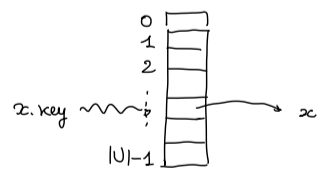
\includegraphics[width=0.4\textwidth]{image/HashTable.png} \\ \\
    \end{tabular}
\end{center}

\paragraph{Problemi:}
\begin{itemize}
    \item Non è possibile avere oggetti con la stessa chiave
    \item OK se il numero $|U|$ è piccolo
\end{itemize}

\begin{mdframed}
\begin{lstlisting}[mathescape=true]
INSERT(T,x)
1   T[x.key] = x        $\Theta(1)$
\end{lstlisting}
\end{mdframed}
\begin{mdframed}
\begin{lstlisting}[mathescape=true]
DELETE(T,x)
1   T[x.key] = NULL     $\Theta(1)$
\end{lstlisting}
\end{mdframed}
\begin{mdframed}
\begin{lstlisting}[mathescape=true]
SEARCH(k)
1   return T[k]         $\Theta(1)$
\end{lstlisting}
\end{mdframed}

\newpage
\subsection{Esempio}
\paragraph{Problema:} consideriamo che la key sia di 8 caratteri (8 bit per rappresentare un carattere). Risulta molto costosa in termini di memoria la tabella hash.
\paragraph{Obiettivo:} usare quantità di memoria proporzionale al numero di elementi da memorizzare.
\paragraph{Idea:} creazione di una tabella $T$ di dimensione $m << |U|$
\begin{equation*}
    h: U \rightarrow \{0, 1, \dots, m-1\}
\end{equation*}
Se $n>m \Rightarrow \exists\; x_1,x_2:h(x_1.key) = h(x_2.key) \Rightarrow$ conflitto \\~\\
Dove:
\begin{itemize}
    \item $n = $ \# elementi memorizzati nella tabella $T$
    \item $m = $ \# celle
\end{itemize}

La collisione verifica con $n = $ numero di elementi memorizzati se $m <<|U|$ se $n > m$. \\~\\

Il principio è il pigeonhole principle, quindi nella tabella hash, ogni valore trova una corrispondenza. 
Il pigeonhole principle è una delle idee più semplici ma più utili della matematica e può aiutarci in questo caso. 
Una versione di base dice che se ($N+1$) piccioni occupano $N$ buche, allora in qualche buca devono esserci almeno 2 piccioni. 
Quindi, se 5 piccioni occupano 4 buche, deve esserci una buca con almeno 2 piccioni.

\subsection{Chaining}
Il Chaining propone come soluzione quella di mettere sulla tabella liste dinamiche di elementi, invece che singoli elementi, in modo che in caso si incorra in una cella già occupata dopo un hashing, l'elemento venga inserito in coda (o in testa) alla lista. Nell'approccio di concatenamento, la tabella hash è una matrice di elenchi collegati, cioè ogni indice ha un proprio elenco collegato.Tutte le coppie chiave-valore mappate allo stesso indice saranno memorizzate nell'elenco collegato di quell'indice.

\begin{center}
    \begin{tabular}{c}
        \\ 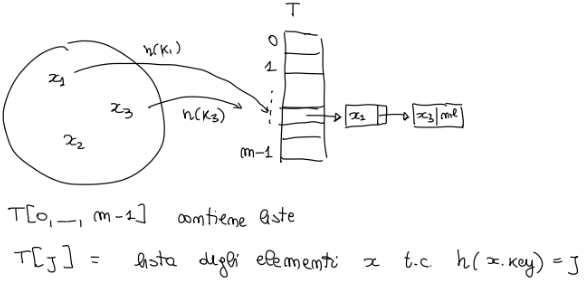
\includegraphics[width=0.7\textwidth]{image/Chaining.png} \\ \\
    \end{tabular}
\end{center}

\newpage
\begin{mdframed}
\begin{lstlisting}[mathescape=true]
INSERT(T,x)
1   T[x.key] = x           $\Theta(1)$
\end{lstlisting}
\end{mdframed}
\begin{mdframed}
\begin{lstlisting}[mathescape=true]
DELETE(T,x)
1   T[h(x.key)] = NULL     $\Theta(1)$
\end{lstlisting}
\end{mdframed}
\begin{mdframed}
\begin{lstlisting}[mathescape=true]
SEARCH(k)
1   return T[h(k)]         $\Theta(n)$
\end{lstlisting}
\end{mdframed}
L'operazione peggiore è quella di ricerca, dove alla peggio la complessità è lineare.

\subsection{Caso medio}
\paragraph{Partenza:}
\begin{itemize}
    \item $m =$ \# celle tabella
    \item $n =$ \# elementi inseriti
    \item $\alpha = \frac{n}{m}$ che può essere minore, maggiore oppure uguale ad 1
\end{itemize}

Ogni elemento $x$ in input ha la stessa probabilità di $\frac{1}{m}$ di essere "indirizzato" in una qualunque delle $m$ celle. Esso è indicato come $n_j =$ lunghezza lista in $T[j]$.

\begin{center}
    \begin{tabular}{c}
        \\ 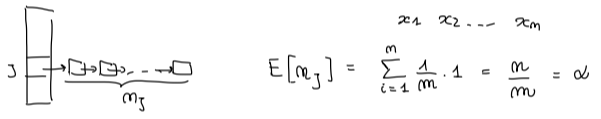
\includegraphics[width=0.7\textwidth]{image/ChainingCasoBase.png} \\ \\
    \end{tabular}
\end{center}

\paragraph{Costo medio di Search:} dato dalla ricerca di una chiave non presente $k$ \\~\\
$\begin{rcases}
    \begin{rcases}
        \text{calcolo } h(k) = j \\
        \text{accedo alla lista } T[j]
    \end{rcases}
    \Rightarrow O(1) \\
    \text{scorro la lista } T[j] \text{ fino in fondo } (n_j \text{elementi}) \Rightarrow n_j
\end{rcases} \Rightarrow \Theta(1 + \alpha)$

\paragraph{Ricerca di una chiave:} presente \\~\\
$\begin{rcases}
    \begin{rcases}
        \text{calcolo } h(k) = j \\
        \text{accedo alla lista } T[j]
    \end{rcases}
    \Rightarrow O(1) \\
    \text{scorro la lista } T[j] \text{ fino in a trovare l'elemento con chiave } k
\end{rcases} \Rightarrow 1+\frac{n_j}{2} \Rightarrow 1+\frac{\alpha}{2}$ \\~\\

Più precisamente: cerco $x$ con chiave $x.key = k$.
